%!TEX root = proyecto.tex

\chapter{Diseño y resolución}

\linespread{1.5}

\section{Paul Viola and Michael Jones}

En 2001, el reconocimiento facial tuvo su primera aparición en el campo de la visión artificial como aplicación en tiempo real. Este avance fue de la mano de Paul Viola y Michael Jones. Análogamente, el punto de partida del estudio de este TFG. Durante este apartado, se estudiará el funcionamiento del algoritmo \textit{Viola-Jones face detector}, ideado por estos dos investigadores y se realizará una implementación del mismo mediante \textit{Python} y \textit{OpenCV} para comprobar como se comporta en la situación actual.

\subsection*{Método de estudio}

El trabajo de los expertos fue presentado por parte de la Universidad de Cambridge mediante un \textit{paper} (ensayo de la investigación). Y se introduce como: 
\begin{quote}
	"This paper describes a machine learning approach for visual object detection which is capable of processing images extremely rapidly and achieving high detection rates" \cite{paulViola}
\end{quote}

Para poder lograr esta afirmación se basan en un procedimiento de trabajo en dos fases: entrenamiento y detección. Igualmente, Paul y Michael dividen el proyecto en tres ideas principales para poder lograr un detector que se pueda ejecutar en tiempo real. Y estas son: la imagen integral, Adaboost (algoritmo de Machine Learning) y un método llamado \textit{attentional cascade structure}. 

Con todos estos puntos combinados lograron ingeniar un prototipo capaz de detectar caras humanas con un \textit{frame rate} de 15 fps. Fue diseñado para la detección de caras frontales, haciendose difícil para posiciones laterales o inclinadas.

Las imagenes que se toman para realizar la detección pasan por una transformación del espacio de color a \textit{grayscale}. Con el objeto de encontrar caracteristicas en ellas, llamadas \textit{haar-like features}. Nombradas así por su inventor Alfred Haar en el siglo XIX. En este trabajo se hacen uso de tres tipos de haar-like features, que son las siguientes:

\begin{figure}[htp]
	\centering
	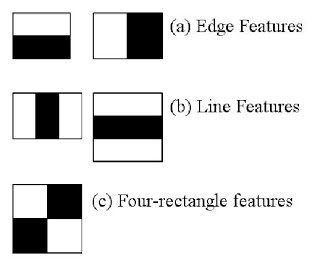
\includegraphics[width=5cm]{imagenes/haar-like.jpeg}
	\caption{Haar-like Features}
	\label{fig:haarLike}
\end{figure}

Las \textbf{\textit{Haar-like features}}, o también conocidas como \textit{Haar-wavelet} son una secuencia de funciones \textit{rescaled square-shaped}, siendo similares a las funciones de Fourier y con un comportamiento parecido a los \textit{Kernel} usados en las \textit{Redes Convolucionales} (matrices que consiguen extraer ciertas \textit{features} de la imagen de entrada). De manera que, las \textit{Haar Features} serán las características de la detección facial.

En un estudio ideal, los pixeles que forma el \textit{feature} tendra una division clara entre pixeles de color blanco con los de color negro (Figura 4.1), pero en la realidad eso casi nunca se va a dar.

Más especificamente, las \textit{Haar-like features} estan compuestas por valores escalares que representan la media de intensidades entre dos regiones rectangulares de la imagen. Estas capturan la intesidad del gradiente, la frecuencia espacial y las direcciones, mediante el cambio del tamaño, posición y forma de las regiones rectangulares basandose en la resolución que se define en el detector. \cite{haar-like}

Estas características van a ayudar al ordenador a entender lo que es la imagen estudiada. Van a ser utilizadas mediante \textit{Machine Learning} para detectar donde hay una cara o no, mediante un recorrido sobre toda la imagen. Esto conlleva una potencia de computación elevada. Para paliar este problema idearon el método de la \textit{Imagen Integral}.

La \textbf{\textit{Imagen Integral}} permite calcular sumatorios sobre subregiones de la imagen, de una forma casi instantanea. Además de ser muy útiles para las \textit{HAAR-like features}, tambien lo son en muchas otras aplicaciones.

Si se supone una imagen con unas dimensiones de $<w,h>$ (ancho y alto, respectivamente), la imagen integral que la representa tendrá unas dimensiones de $<w+1,h+1>$. La primera fila y columna de esta son ceros, mientras que el resto tendrán el valor de la suma de todos los pixeles que le preceden. \cite{integral-web} Ahora, para caluclar la suma de los pixeles en una region especifica de la imagen, se toma la correspondiente en la imagen integral y se suma según la siguiente fórmula (siguiendo la numeración de la Figura \ref{fig:integral}):
\begin{center}
	$sum = L4 + L1 - (L2 + L3)$ 
\end{center}
\begin{figure}[htp]
	\centering
	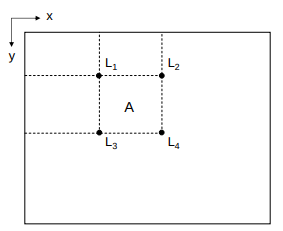
\includegraphics[width=5cm]{imagenes/integral.png}
	\caption{Funcionamiento de una \textit{Imagen Integral}}
	\label{fig:integral}
\end{figure}

Viola y Jones junta esta propuesta con los filtros \textit{Haar-like features}, y consiguen computar dichas características de manera constante y eficaz. \cite{integral}\\

% ---------------------------
%https://aishack.in/tutorials/integral-images-opencv/

%https://www.quora.com/How-integral-image-is-used-in-image-processing-and-how-improves-the-computation-time?share=1
%https://www.quora.com/What-are-the-must-read-papers-in-the-field-of-computer-vision-for-a-student-in-pursuing-research-in-the-field
% ---------------------------
%
% MACHINE LEARNING - ADABOOST
\newpage
Una vez estudiada la obtención de características y con un set de entrenamiento, solo queda seleccionar un método de \textit{machine learning} que permita crear una función de clasificación. Concretamente, se plantea el uso de una variante de \textbf{\textit{AdaBoost}}, que permite seleccionar un pequeño conjunto de características y poder entrenar un clasificador. 

Este algoritmo de aprendizaje esta basado en generar una predicción muy buena a partir de la combinación de predicciones peores y más débiles, donde cada uno de estas se corresponde con el \textit{threshold} de una de las características \textit{Haar-like}. La primera vez que aparece este algoritmo, de forma práctica, fue de la mano de \textit{Freund y Schapire} \cite{adaboost1}. Sin embargo, el usado por \textit{Viola y Jones} es una modificación de este.

La salida que genera el algoritmo \textbf{\textit{AdaBoost}} es un clasificador llamado \textit{Strong Classifier}, como se ha mencionado anteriormente, compuesto por combinaciones lineales de \textit{Weak Classifiers}. 

El procedimiento para encontrar \textit{Weak Classifiers} es ejecutar el algoritmo T iteraciones donde T es el número de clasificadores a encontrar. En cada iteración, el algoritmo busca el porcentaje de error entre todas las características y escoje la que menos porcentaje de error presente en dicha iteración. (Como se muestra en la \textit{Figura \ref{fig:ada1}}) \cite{adaboost2}

\begin{figure}[htp]
	\centering
	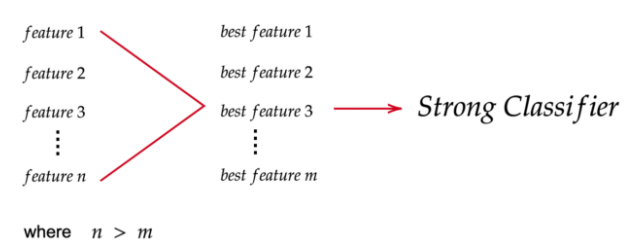
\includegraphics[width=10cm]{imagenes/ada1.png}
	\caption{Construcción del \textit{Strong Classifier}}
	\label{fig:ada1}
\end{figure}

Con estos clasificadores se procede a la construcción de una estructura en cascada para crear un \textit{Multi-stage Classifier}, que podrá realizar una detección rápida y buena. Por tanto, la estructura de cascada esta compuesta por varios estados de \textit{Strong Classifiers} generados por el algoritmo \textit{AdaBoost}. Donde el trabajo de cada estado será identificar si, dada una región de la imagen, no hay una cara o si hay la posibilidad de que la haya. \cite{adaboost1}

Si el resultado de uno de los estados es que no existe una cara en dicha región, esta se descarta directamente. Mientras que, si hay la posibilidad de que exista una, pasa al siguiente estado de la estructura. De tal forma que, cuantos más estados atraviese una región de la imagen, con más seguridad se podrá afirmar que existe una cara en ella. La estructura completa se refleja en la \textit{Figura \ref{fig:ada2}}.

\begin{figure}[htp]
	\centering
	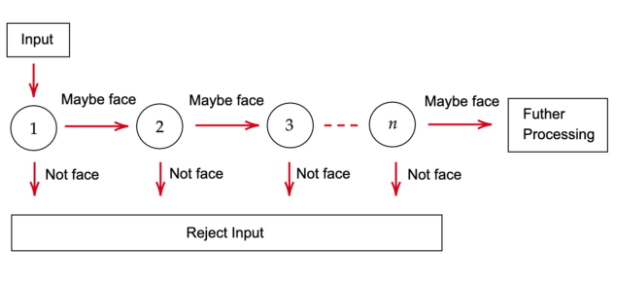
\includegraphics[width=10cm]{imagenes/ada2.png}
	\caption{Construcción del \textit{Multi-stage Classifier}}
	\label{fig:ada2}
\end{figure}

% VIDEO DE LOCOS: https://www.youtube.com/watch?v=uEJ71VlUmMQ&t=5s

\subsection*{Implementación y Experimentación}

\begin{itemize}
	\item Explicar su funcionamiento
	\item Mostrar funcionamiento y aplicacion al objetivo
\end{itemize}



\section{HOG y Dlib}

\begin{itemize}
	\item Explicar su funcionamiento
	\item Mostrar funcionamiento y aplicacion al objetivo
\end{itemize}

\section{Facial Landmask}

\begin{itemize}
	\item Explicar su funcionamiento
	\item Mostrar funcionamiento y aplicacion al objetivo
\end{itemize}

\section{Facial Landmask Custom}

\begin{itemize}
	\item Plantear idea
	\item Proceso de creacion
	\item Mostrar funcionamiento y aplicacion al objetivo
\end{itemize}

\section{YOLO}

\begin{itemize}
	\item Acercamiento al Deep Learning
	\item Explicar su funcionamiento
	\item Mostrar funcionamiento y aplicacion al objetivo
\end{itemize}

\section{Tensorflow}

\begin{itemize}
	\item Plantear idea
	\item Procedimiento
	\item Mostrar funcionamiento y aplicacion al objetivo
\end{itemize}